\documentclass[brazil,hardcopy,openany,a5paper]{ufscthesis}
\usepackage[brazil]{babel}
\usepackage{amsfonts, amsmath, amsthm, amsbsy,amssymb,bm,mathtools} % For math fonts, symbols and environments %
\usepackage{graphicx} 		% Required for including images
\usepackage{transparent}	% may be required for inkscape pdf figures (http://bit.ly/18i5Oga)
\usepackage{listings}
\usepackage[abnt-emphasize=bf]{abntex2cite}
\usepackage{caption}
\usepackage{multirow}
\usepackage{lscape}
\usepackage[T1]{fontenc}
\sloppy
\usepackage{siunitx}
\usepackage{nameref}
\usepackage{float}

\newcommand{\source}[1]{\small \caption*{Fonte: {#1}} } % Criar fonte embaixo da figura

\newsubfloat{figure}		% Allow subfloats in figure environment (http://bit.ly/1C20NAj)
\graphicspath{{figures/}} 	% Location of the graphics files

\usepackage{siunitx} % units package
\let\DeclareUSUnit\DeclareSIUnit
\let\US\SI
\let\us\si
\DeclareUSUnit\inch{in}
\sisetup{detect-all}  %it may be necessary to load it after loading the font package

\citebrackets[]

%----------------------------------------------------------------------
% Comandos criados pelo usuário
\newcommand{\afazer}[1]{{\color{red}{#1}}} % Para destacar uma parte a ser trabalhada
\DeclareMathOperator*{\argmin}{\arg\!\min}
\DeclareMathOperator*{\argmax}{\arg\!\max}


%----------------------------------------------------------------------
% Identificadores do trabalho
% Usados para preencher os elementos pré-textuais
\instituicao[a]{Universidade Federal de Santa Catarina} % Opcional
\departamento[a]{Biblioteca Universitária}
\programa[o]{Programa de Pós-Graduação em Engenharia Civil} 
\curso{Engenharia de Engenharia Civil}
\documento[a]{Dissertação} % [o] para dissertação e trabalho de conclusão de curso [a] para tese
\grau{Mestre} % doutor, mestre, engenheiro, etc.
\titulo{Modelagem do impacto da ilha de calor sobre o desempenho energético de escritórios condicionados artificialmente}
\subtitulo{} % Opcional
\autor{Marcelo Salles Olinger}
\local{Florianópolis} % Opcional (Florianópolis é o padrão)
\data{24}{junho}{2019}
\orientador[Universidade Federal de Santa Catarina]{Profa. Ana Paula Melo, Dra.}
\coordenador[Universidade Federal de Santa Catariana]{Prof. Fulano de Tal, Dr.}
\orientadornabanca{sim} % Se faz parte da banca definir como sim
\coorientadornabanca{nao} % Se faz parte da banca definir como sim
\bancaMembroA{Prof. Saulo Guths, Dr.\\Universidade Federal de Santa Catarina}  %Nome do presidente da banca
\bancaMembroB{Prof. Membro Dois, Dr.\\Universidade Federal de Santa Catarina}   % Nome do membro da Banca
\bancaMembroC{Profa. Membro Três, Dra.\\Outra Universidade} % Nome do membro da Banca
% \bancaMembroD{Quarto membro\\Universidade ...} % Nome do membro da Banca
% \bancaMembroE{Quinto membro\\Universidade ...}  % Nome do membro da Banca
% \bancaMembroF{Sexto membro\\Universidade ...}   % Nome do membro da Banca
% \bancaMembroG{Sétimo membro\\Universidade ...}  % Nome do membro da Banca

%\dedicatoria{Dedico essa conquista aos amigos e familiares que tornaram isso possível.}

%\agradecimento{Inserir os agradecimentos aos colaboradores à execução do trabalho. Inserir os agradecimentos aos colaboradores à execução do trabalho.}

%\epigrafe{Se você pensa que pode ou se pensa que não pode, de qualquer forma você está certo.}{Henry Ford}

\textoresumo {
O condicionamento de ar para resfriamento de edificações é responsável por parcela significativa do consumo energético, e tende aumentar nas próximas décadas. Uma solução para a mitigação do aumento no consumo de energia para resfriamento é a ventilação natural (VN). A VN é uma técnica muito presente em países de clima quente, onde possui um grande potencial de aplicação. Para que seja aplicada de forma efetiva e otimizar seu potencial, é importante que a VN seja concebida desde a fase inicial de projeto. Durante a fase inicial de projeto, há pouco detalhamento relacionado ao projeto arquitetônico, e há necessidade de agilidade nas tomadas de decisão. Diante deste cenário, uma ferramento capaz de predizer o conforto térmico em edificações de forma simples e rápida pode ser de grande utilidade.

O objetivo deste estudo é desenvolver um metamodelo de rede neural artificial capaz de predizer o conforto térmico em escritórios de edificações ventiladas naturalmente. 

O indicador de conforto térmico utilizado é a fração de horas do ano em que há desconforto térmico por calor no ambiente, de acordo com o método adaptativo da ASHRAE Standard 55 (2017), para 80\% de aceitabilidade entre os ocupantes.

O metamodelo é desenvolvido a partir de uma base de dados de simulações termo-energéticas obtidas através do programa computacional EnergyPlus. O método de amostragem é o Hipercubo Latino. Os modelos que compõem a base de dados foram definidos a partir das características comumente encontradas em edificações de escritórios da cidade de São Paulo. A definição dos parâmetros variados no desenvolvimento dos modelos é estabelecida através da análise de sensibilidade global de Sobol.

O treinamento da rede neural artificial é realizado com  80\% dos casos da base de dados. Os casos restantes são utilizados para a validação do metamodelo. Os indicadores de desempenho do metamodelo são o erro médio quadrático (RMSE) e o coeficiente de determinação (R$^2$).

Como resultado, espera-se obter um metamodelo capaz de predizer, com boa precisão, a fração de horas de desconforto por calor em escritórios ventilados naturalmente.
}
\palavraschave{Ventilação natural. Metamodelo. Simulação termoenergética de edificações.}

\textabstract {Text...}
\keywords{Word 1. Word 2. Word 3.}

\begin{document}

	
	%--------------------------------------------------------
	\frontmatter
	% Elementos pré-textuais
	\folhaderosto[pre/Ficha_Catalografica.pdf]
	\folhadeaprovacao{}{} %{pre/signature_page_color.pdf}{}
	%\paginadedicatoria
	%\paginaagradecimento
	%\paginaepigrafe
	\paginaresumo
	\paginaabstract
	% ---
	\listadefiguras % as listas dependem da necessidade do usuário
	\listadetabelas 
	%\listadeabreviaturas
	%\listadesimbolos
	\sumario
	%--------------------------------------------------------
	\mainmatter

	\chapter{Introdução}
\label{chapter:introducao}

%como referenciar o paragrafo inteiro?
A demanda de energia para o resfriamento de ar em edificações mais que triplicou do ano de 1990 a 2016 (IEA, 2018). De acordo com a Agência Internacional de Energia, o consumo de energia elétrica global destinado ao resfriamento de edificações em 2016 foi de 2.020 TWh/ano, correspondendo a quase um quinto do consumo total no setor. Se não houver mudanças no cenário atual, estima-se que a demanda por energia para resfriamento mais que triplicará até o ano de 2050, representando 37\% do aumento no consumo de eletricidade em edificações. Isso corresponderá a 11,5\% do consumo de energia total em edificações comerciais. Esse cenário é ainda mais impactante em países de clima quente, com economias emergentes. Das 2,8 bilhões de pessoas que vivem nas partes mais quentes do mundo hoje, apenas 8\% possui condicionamento de ar para resfriamento. No Brasil, a parcela do resfriamento de ar nas cargas de pico das redes elétricas em 2016 correspondia a 7,6\% do total. Até o ano de 2050, essa parcela pode representar 30,8\% da carga de pico, se nenhuma medida for tomada para a mitigação do problema.

O crescimento econômico e populacional aumentam a demanda de energia. Essa demanda pode causar grandes impactos ambientais, como poluição, alterações climáticas e esgotamento dos recursos naturais. Para garantir a melhora na qualidade de vida de forma sustentável, busca-se políticas de incentivo à eficiência energética. No Brasil, desde 2009 o INMETRO possui um programa de etiquetagem de edificações voltado para padrões de eficiência energética de edificações (BRASIL, 2009).

A redução dos impactos ambientais relacionados ao resfriamento de edificações pode ser alcançada através da geração de energia proveniente de fontes renováveis, do desenvolvimento de equipamentos com maior eficiência energética, ou pela busca de soluções passivas. O resfriamento passivo é um conjunto de técnicas sustentáveis para resfriar edifícios por meios naturais (SAMANI et al., 2016). Consiste em qualquer sistema que busca minimizar, ou eliminar se possível, o uso de sistemas de condicionamento de ar. Técnicas de resfriamento passivo têm o objetivo de reduzir as altas temperaturas internas e o consumo de energia para resfriamento, proporcionando conforto térmico para os ocupantes.

Uma das técnicas de resfriamento passivo é a ventilação natural (VN). A VN como estratégia para resfriamento de edificações é um dos componentes fundamentais no desenho de edifícios energeticamente eficientes. Técnicas de VN são encontradas ao longo de toda a história, e hoje vêm sendo atualizadas de acordo com novos estudos no campo de conforto térmico e desenhos sustentáveis de edificações (PESIC; CALZADA; ALCOJOR, 2018). Além de assegurar a qualidade do ar, a ventilação natural promove o resfriamento da edificação, proporcionando conforto térmico aos usuários quando as condições do clima externo são favoráveis (YAO et al., 2009).

Para que o conforto térmico dos usuários seja garantido sem um consumo significativo de energia, é importante entender como ocorrem as variações térmicas em um edifício antes de construí-lo. Análises durante os estágios iniciais de projeto de uma edificação com VN podem apontar decisões fundamentais para o desempenho térmico. No estágio inicial de projeto, o potencial de otimização é maior e nesta etapa qualquer estimativa da influência dos ocupantes no conforto e desempenho energético pode fazer diferença nas tomadas de decisão (BELLERI; LOLLINI; DUTTON, 2014; ROETZEL; TSANGRASSOULIS; DIETRICH, 2014).

Atualmente, a forma mais avançada de predição do desempenho energético de edificações é a simulação computacional. Porém, simulações energéticas dinâmicas requerem modelos detalhados e enfrentam diversos problemas associados principalmente a informações necessárias para dados de entrada do modelo processado (CORGNATI et al., 2013). Através do uso de metamodelos, é possível obter resultados próximos aos de simulações de desempenho energético complexas, facilitando sua aplicação em diversas áreas.

Metamodelos para eficiência energética de edificações podem ser desenvolvidos a partir de diversos métodos (ØSTERGÅRD; JENSEN; MAAGAARD, 2018). A solução mais apropriada depende do contexto e propósitos de cada aplicação. O desenvolvimento de um metamodelo capaz de estimar conforto térmico em edificações comerciais já foi proposto por \citeauthoronline{Rackes2016} \cite{Rackes2016}. Voltado principalmente a tipologias de escolas, o metamodelo estima a fração de horas de ocupação em que os ocupantes sentiriam desconforto por calor ao longo do ano, através do modelo de máquina de vetores de suporte.

A avaliação do potencial de resfriamento por VN em edificações apresenta desafios, por apresentar comportamentos complexos e fazer-se necessária desde a fase inicial de projeto. Por meio de ferramentas de aprendizagem automática, surge a possibilidade do desenvolvimento de metamodelos capazes de obter resultados de conforto térmico em edificações de forma simples e rápida.

\section{Objetivos}
\subsection{Objetivo geral}

O objetivo deste estudo é desenvolver um metamodelo por meio de rede neural artificial, capaz de estimar o conforto térmico em edifícios de escritórios ventilados naturalmente.

\subsection{Objetivos específicos}

Dentre os objetivos específicos deste trabalho estão:

\begin{itemize}
	\item identificar o universo de possíveis características encontradas em edifícios de escritórios ventilados naturalmente no Brasil;
	\item definir as variáveis com maior e menor influência no desempenho térmico dos edifícios ventilados naturalmente;
	\item explorar formas de simplificar um modelo de edifícios para que possa ser representado com apenas uma zona térmica.
\end{itemize}
	
	\section{Estrutura do trabalho}
	
	Lorem ipsum dolor sit amet, consectetur adipiscing elit. Nulla commodo, augue non consectetur vehicula, felis velit commodo eros, nec bibendum augue purus quis mi. Donec dapibus id magna eget euismod. In lacinia porttitor velit, in lacinia erat commodo et. Nulla feugiat posuere ipsum, eu euismod lorem efficitur ut. Sed dapibus lobortis ex, eu vehicula sem dignissim nec. Phasellus pellentesque tellus vitae tortor consectetur volutpat. Proin pulvinar lectus id tellus congue maximus.

	Sed semper arcu at posuere scelerisque. Pellentesque a lorem eu lorem lobortis cursus aliquam ut diam. Ut tristique, lacus eget gravida euismod, ante nisl elementum elit, a efficitur neque est eu tellus. Phasellus in convallis tortor. Nullam auctor auctor tempus. Pellentesque placerat, est at convallis congue, velit sapien tempor orci, eu eleifend nisi purus sed odio. Duis nec rhoncus enim. Nunc vitae consectetur sapien. Nullam in enim iaculis, laoreet ex in, aliquet massa. Nulla facilisi. Sed vulputate eros et mi imperdiet, nec commodo libero tristique. Mauris vel pretium felis. Suspendisse feugiat tortor vitae dapibus semper. Fusce dignissim est eget mattis auctor.

\chapter{Revisão de literatura}
	
	\section{Ventilação natural}
	
	A ventilação natural (VN) ocorre quando diferenças de pressão geradas pelo vento ou por forças de empuxo agem em uma ou mais aberturas da envoltória de uma edificação \cite{CarrilhodaGraca2016}. Um sistema de VN pode ser caracterizado pela estratégia de ventilação, a locação das aberturas e as suas áreas. Apesar de muitos regulamentos exigirem uma área mínima de ventilação, tipicamente definida em função da área de piso, essas são grandes simplificações. A área de abertura ideal depende do tipo de sistema (unilateral ou cruzada), do clima e dos objetivos relacionados ao período de uso da VN.
	
	A VN pode ser aplicada por meio de grelhas, sistemas de dutos, ou simplesmente grandes aberturas, como janelas ou portas. No caso de grandes aberturas, duas configurações podem ser consideradas: ventilação cruzada, ou ventilação unilateral. Diferentemente da ventilação cruzada, a turbulência do vento e as variações nos gradientes de pressão induzidos por rajadas podem afetar fortemente o fluxo de ar em uma abertura unilateral. Como esses parâmetros não são estáveis, é mais complicado avaliar a ventilação unilateral (FREIRE; ABADIE; MENDES, 2013). Carrilho da Graça e Linden (2016) apontam que para otimização da VN unilateral em edificações pequenas ou médias, para
	a mesma área total de abertura, duas ou mais aberturas são mais eficientes do que apenas uma, sendo que aberturas espaçadas funcionam melhor do que próximas.
	
	Além das diferentes estratégias relacionadas à configuração das aberturas na edificação, há também diferentes abordagens quanto aos períodos de funcionamento. Algumas edificações podem permitir o uso da VN durante o dia, enquanto outras também permitem o uso de VN noturna. Há também casos em que a VN é exclusivamente noturna, e durante o dia utiliza-se sistemas de condicionamento de ar (PESIC; CALZADA; ALCOJOR, 2018).
	
	O mecanismo de ventilação natural noturna é baseado na transferência de calor por convecção da estrutura exposta do edifício para o fluxo de ar frio da noite (momento em que a diferença entre a temperatura do ar interno e externo é maior) (BREESCH; JANSSENS, 2010). Durante o dia, a massa térmica da	edificação é utilizada para acumular os ganhos de calor internos e do sol, e prevenir condições desconfortáveis durante as horas de operação da edificação.
	
	Isso leva a três consequências: para garantir o funcionamento, o calor deve ser armazenado na estrutura da edificação, e é necessário garantir uma ponte para que haja a transferência de calor para/da estrutura; a ventilação noturna é mais apropriada para climas moderados e frios, com maiores diferenças diárias de temperatura ao longo do dia; como essa tecnologia utiliza apenas calor sensível, é menos aplicável em climas quentes e úmidos.
	
	Prover, efetivamente, VN em edifícios pode economizar energia e custo em comparação à ventilação mecânica devido à baixa manutenção e custo zero de operação (OMRANI et al., 2017). O desempenho da VN é medido, primariamente, através de parâmetros de dinâmica dos fluidos, como padrão do fluxo de ar, velocidade média, taxa de fluxo de ar, distribuição de pressão, renovações de ar, fluxo volumétrico e outras qualidades que podem ser derivadas desses parâmetros. Esses elementos do fluxo também podem ser usados para determinar características mais amplas do ambiente interno de edificações, como a qualidade do ar e conforto térmico. Há muitos métodos de
	avaliação de desempenho de VN, cada um com suas vantagens e limitações. O método escolhido deve ser o mais apropriado, baseado nos recursos, exigências e estágio do projeto.
	
	Estimar o desempenho da VN no projeto da edificação envolve a consideração de fenômenos físicos complexos, o que pode ser dificultoso. Para a simulação computacional, há duas principais formas de descrever a ventilação natural: Computer Fluid Dynamics (CFD) e Airflow Network (AFN). O CFD utiliza equações de Navier-Stokes para resolver diretamente o problema do fluxo de ar através das propriedades da dinâmica dos fluidos (ARENDT; KRZACZEK; TEJCHMAN, 2017). Apesar do grande custo computacional, o CFD disponibiliza informações detalhadas sobre a distribuição da velocidade do ar, temperatura, pressão e concentração de partículas na área analisada. No entanto, bons
	resultados com o uso dessa ferramenta dependem da qualidade da grade adotada, aplicação correta das condições de contorno, e aplicação correta das diversas suposições tomadas na aplicação do modelo. Já o AFN funciona a partir de uma rede de nós, análoga a um circuito
	elétrico. A cada zona térmica da edificação é atribuído um nó, e os caminhos do fluxo recebem uma resistência equivalente para cada ligação entre as zonas.
	
	Condições dentro da zona, como velocidade do ar, temperatura, umidade são então computadas com base nas diferenças de pressão entre as zonas definidas e são comumente resolvidas em condições estacionárias (OMRANI et al., 2017).
	
	O uso de modelos multi-zona exige a suposição de que o ar dentro de cada zona é homogêneo, com temperatura, velocidade, concentração de contaminantes e umidade relativa uniformes. Modelos multi-zona são úteis na predição do desempenho de VN do edifício como todo, por prover resultados robustos. Porém, não podem prover informações detalhadas sobre o comportamento do
	ar dentro da zona. Apesar de ser uma abordagem muito mais simplificada, o AFN é muito utilizado em razão da facilidade de aplicação e por ter um custo computacional muito mais baixo, quando comparado ao CFD. Ferramentas de simulação computacional como EnergyPlus podem integrar o modelo térmico de um edifício com um modelo AFN (BELLERI; LOLLINI; DUTTON, 2014).
	
	O modelo de pressão e fluxo de ar utilizado pelo EnergyPlus (2018) foi desenvolvido baseado no modelo AIRNET (WALTON, 1989). Os cálculos de fluxo de ar multi-zona são realizados no timestep do sistema HVAC (Heating, Ventilation and Air-Conditioning). O modelo de rede de fluxo de ar consiste em três passos sequenciais:
	
	1- cálculos de pressão e fluxo de ar;
	
	2- cálculos de temperatura e umidade no nó;
	
	3- cálculos de carga sensível e latente.
	
	Os cálculos de pressão e fluxo de ar determinam, a partir das pressões de vento e fluxos de ar forçados, a pressão em cada nó e o fluxo de ar através de cada ligação. Baseando-se no fluxo de ar calculado para cada ligação, o modelo	calcula as temperaturas e umidades relativas em cada nó a partir das temperaturas e umidades relativas das zonas. Utilizando as temperaturas e umidades relativas calculadas, as cargas latentes e sensíveis conduzidas pelos	sistemas de fluxo forçado e das infiltrações são somadas em cada zona. As cargas latentes e sensíveis obtidas nessa etapa são utilizadas então nas equações de balanço energético das zonas para predizer possíveis cargas relacionadas ao sistema HVAC e calcular as temperaturas do ar, umidades relativas e pressões finais da zona.
	
	Uma ligação utilizada no modelo no AFN tem dois nós, um de entrada e um de saída, e possui um componente que determina a relação entre o fluxo de ar e a pressão. A diferença de pressão entre cada componente em uma ligação é calculada pela equação de Bernoulli. Como apresentado na Figura 2.1, cada nó é atribuído a uma zona e cada ligação corresponde a um elemento de resistência entre os nós, que pode representar uma abertura, ou uma superfície com frestas.
	
	Figura 2.1 - Relação entre nós e ligações
	
	Fonte: EnergyPlus (2018).
	
	A velocidade na qual considera-se que o vento atinge a edificação modelada é obtida a partir do arquivo climático utilizado na simulação
	computacional. A partir das medições de velocidade do vento na estação meteorológica, extrapola-se os valores para as outras altitudes e os perfis de terreno. Essa consideração em relação à velocidade do vento é baseada no
	Handbook of Fundamentals da ASHRAE (2005).
	
	Os coeficientes do perfil de velocidade do vento são variáveis que dependem das características de rugosidade do terreno no entorno. Os valores típicos são apresentados na Tabela 2.1.
	
	Tabela 2.1 - Coeficientes do perfil de velocidade do vento 
	
	Fonte: ASHRAE (2005).
	
	O valor padrão para a medição da velocidade de vento é de 10 m de altitude. Os valores padrão para $\alpha_{met}$ e $\delta_{met}$ são 0,14 e 270 m, respectivamente, porque a maioria das estações meteorológicas estão localizadas em campos abertos.
	
	Ao definir a velocidade do vento, o programa EnergyPlus calcula a pressão do vento sobre as edificações, determinada também pelo princípio da equação de Bernoulli.
	
	A maior dificuldade no desenvolvimento do AFN é a necessidade de estimar as características do fluxo nas aberturas e o coeficiente de pressão do vento na edificação (ARENDT; KRZACZEK; TEJCHMAN, 2017). Os coeficientes de pressão do vento (Cp) descrevem como o vento interfere na distribuição externa de pressões em volta da edificação. Os Cp dependem principalmente da geometria da edificação, dos detalhes da fachada, do entorna da edificação, da velocidade e direção do vento, e da intensidade da turbulência. Na prática,
	destaca-se a dificuldade em determinar precisamente a relação entre o Cp e todos esses fatores. As abordagens mais realistas são os experimentos em escala real in-situ. No entanto, esses experimentos possuem custo elevado e normalmente possuem grandes incertezas. Os dados dos Cp podem ser estimados das seguintes fontes: testes de túnel de vento; simulações com CFD; modelos analíticos; e bases de dados.
	A dificuldade em se considerar toda a complexidade de variação do Cp faz com que os programas de simulação termo-energética de edificações com AFN, geralmente, incorporem métodos simplificados (CÓSTOLA; BLOCKEN; HENSEN, 2009). Os experimentos de túnel de vento são as fontes primárias mais comuns. A qualidade dos resultados de túneis de vento são diretamente afetados pela calibração do túnel de vento, a garantia de qualidade dos procedimentos, e os conhecimentos do pessoal para a preparação e execução dos testes.
	
	Os túneis de vento oferecem um bom grau de controle sobre os experimentos, assim como a repetitividade e reprodutibilidade dos testes conduzidos (OMRANI et al., 2017). No entanto, a escala pode afetar o fluxo de ar e as transferências de calor se os parâmetros adimensionais corretos não são mantidos entre os modelos de diferentes tamanhos. Portanto, o ideal é usar modelos em escala real.
	Em casos em que não é possível obter os valores de Cp por fontes primárias, Cóstola, Blocken e Hensen (2009) apontam as bases de dados como as fontes secundárias mais comuns. A base de dados de pressão de vento da Universidade Politécnica de Tóquio oferece dados experimentais obtidos a partir de experimentos em túnel de vento (TPU, 2018). A base de dados possui os resultados de testes conduzidos utilizando-se modelos de acrílico em um túnel de vento de seção de 2,2 m de largura por 1,8 m de altura. A camada limite
	atmosférica foi simulada por elementos geradores de turbulência e outros elementos de rugosidade. Diferentes perfis de vento foram usados para construir a base de dados. Na maioria dos experimentos a velocidade média e os perfis de intensidade de turbulência estavam de acordo com as de terreno suburbano. A intensidade de turbulência à altura de 10 cm foi cerca de 0,25, e a velocidade de vento teste a essa altura foi 7,4 m/s. O número mínimo de Reynolds foi 25340, que é acima do limite 11000 para o fluxo independente.
	
	Diversos fatores que afetam o valor do Cp são comumente simplificados, como apontado por Cóstola et al. (2010) no Quadro 2.1.
	
	Quadro 2.1 - Fatores que afetam o Cp e simplificações comuns
	
	Fonte: Cóstola et al. (2010)
	
	De acordo com Cóstola et al. (2010), os Cp médios se definem de acordo
	com Equação 2.1 e Equação 2.2.
	
	Onde:
	
	Px é a pressão estática em um dado ponto da fachada do edifício (Pa);
	P0 é a pressão estática de referência (Pa);
	Pd é a pressão dinâmica (Pa);
	$\rho$ é a densidade do ar (kg/m3);
	Vref é a velocidade do vento de referência.
	
	Nas simulações termo-energéticas de edificações, há muita incerteza relacionada ao Cp. Isso deve-se à influência do Cp em muitos dos indicadores de desempenho, como consumo de energia ou conforto térmico, que são frequentemente sensíveis à taxa de fluxo de ar (CÓSTOLA; BLOCKEN; HENSEN, 2009). Bases de dados de Cp são compilações de uma ou mais fontes, onde os dados são classificados de acordo com alguns parâmetros, como a forma da edificação e a orientação de incidência do vento. As bases de dados de Cp são amplamente disponíveis, particularmente para o cálculo de carga de vento em estruturas. Esses valores de Cp para edificações sem obstruções, com geometria simples, podem ser utilizados quando experimentos em túneis de vento não são disponíveis. Uma abordagem similar é usada para bases de dados de ventilação e infiltração na literatura. Nenhuma das bases de dados e modelos analíticos lidam com os efeitos da topografia local, detalhes da fachada, ou informam a incerteza dos dados disponibilizados. Os efeitos das edificações do entorno são considerados com muitas limitações e simplificações.
	
	O estudo de Cóstola et al. (2010) quantifica a incerteza na taxa de fluxo de ar devido ao uso do Cp médio da fachada, considerando 15 formas de edifícios e diferentes configurações de aberturas. O foco era em ventilação e infiltração movidas por vento, e a força de empuxo não foi considerada. Este estudo apresentou a estimativa de incerteza para edificações com duas aberturas idênticas, e uma zona interna, baseando-se em uma grande faixa de formas e ângulos de incidência do vento. A incerteza na taxa de fluxo de ar calculadas usando-se os coeficientes médios da superfície para edificações isoladas com duas aberturas variam entre 0,23 e 5,05 vezes o fluxo comparadas ao uso do Cp local, para um intervalo de confiança de 95\%. As grandes incertezas relativas devem-se às pequenas taxas de fluxo de ar. Quando considera-se apenas as superfícies com maiores diferenças de pressão relativa, a incerteza diminui para  valores entre 0,52 e 1,42 vezes. Conclui-se que a magnitude da incerteza é alta, mas o julgamento em relação a aplicabilidade desses dados depende do problema em análise e do indicador de desempenho escolhido.
	
	O trabalho de Arendt, Krzaczek e Tejchman (2017) estuda a influência dos dados de Cp de diferentes fontes na precisão de um modelo AFN. Uma edificação real com um sistema de ventilação movida por vento e força de empuxo foi adotada para um estudo de caso. Oito casos com diferentes dados de Cp foram estudados. Os resultados de temperatura do ar e fluxo do ar interno foram então comparados com as medições na escala real. Uma edificação residencial de dois pavimentos, localizada em Skarszewy, no norte da Polônia, foi escolhida para o estudo de caso. A edificação possui janelas e chaminés de ventilação. A densidade de construção na área de entorno da edificação não foi especificada no estudo. As simulações foram efetuadas para um período de tempo de 7 dias no fim da primavera. A modelagem da edificação foi realizada através do programa EnergyPlus 8.1(ENERGYPLUS, 2015). Os valores de Cp foram obtidos de duas fontes: CPCALC+, que é um modelo analítico; e AIVC, que oferece uma base de dados. A partir dos dados do AIVC, considerou-se duas possibilidades: área plana aberta; e área rural com barreiras de vento espalhadas. A partir do CPCALC+ considerou-se as seguintes densidades de construção: 1\%, 10\% e 20\%. Para cada densidade de construção utilizada,considerou-se mais um caso onde o Cp para o ângulo de incidência de 180o teve seu valor alterado em -0,1. Essa foi uma variação arbitrária para verificar a influência nos resultados, uma vez que 180o era a direção de incidênciacpredominante do vento no local. Em todos os casos considerou-se o coeficiente de descarga (Cd) das aberturas igual a 0,6. Os casos mais precisos foram: o que considerou os valores da AIVC para terrenos com barreiras esparsas; e o que considerou os valores do CPCALC+ para 1\% de densidade, e variação de -0,1 no Cp para o ângulo de incidência de 180o. O caso mais próximo do real obteve uma diferença relativa de 10\%, enquanto o pior caso (CPCALC+ 1\% dedensidade) obteve um erro relativo de 169\%. Os erros do CPCALC+ foram maiores do que o do AIVC, mesmo considerando-se o Cp para a posição exata da abertura, enquanto o AIVC considerou a média na superfície da fachada. Nos melhores resultados, a diferença calculada para a temperatura do ar foi menor do que 0,5 $^{\circ}$C, enquanto nos piores, foi entre 1,1 $^{\circ}$C e 1,2 $^{\circ}$C. A correlação entre a precisão relativa do fluxo de ar e da temperatura do ar não foi linear. A conclusão final foi que simulações com AFN na fase inicial de projeto, quando não há dados experimentais disponíveis para a validação do modelo, possuemcsignificantes incertezas.
	
	Freire, Abadie e Mendes (2013) avaliaram diferentes modelos de ventilação cruzada e unilateral (British Standard, Gids e Phafe, e Larsen) e compararam com resultados de medições in-situ e em túneis de vento. Também são avaliadas as bases utilizadas para obtenção dos Cp. O modelo de Larsen mostrou-se mais apropriado para a ventilação unilateral, por considerar variações em função do ângulo de incidência do vento. Os Cp do CPCALC (Cp local) obtiveram resultados mais precisos do que os das equações de Swami e Chandra (Cp médio), que é o método padrão do programa EnergyPlus (2018) para a obtenção do Cp. Porém, ambos obtiveram erros relativos por volta de 30\%. O fluxo de ar por grandes aberturas envolve diferentes obstáculos, que inclui desde fluxos gravitacionais estáveis, até fluxos flutuantes devido à turbulência do vento. A solução utilizada pelo programa EnergyPlus 8.9 (ENERGYPLUS, 2018) para a modelagem de grandes aberturas é baseada no modelo COMIS (FEUSTEL; RAYNER-HOOSON, 1990). As principais premissas para esse modelo são:
	
	\begin{itemize}
		\item fluxo estável, fluido não-viscoso e incompressível;
		\item estratificação linear da densidade em ambos lados da abertura;
		\item efeitos de turbulência representados por um perfil de diferença de pressão equivalente;
		\item efeitos de redução da área efetiva de abertura representados por um	coeficiente.
	\end{itemize}
	
	O componente Detailed Opening do EnergyPlus (2018) assume que tanto a diferença de pressão através da abertura, quanto a densidade do ar são função da altura, então é possível haver fluxo de ar em três partes através da abertura, como apresentado na Figura 2.2.
	
	Figura 2.2 - Fenômenos considerado pelo EnergyPlus ao modelar fluxo de ar através de grandes aberturas
	
	Fonte: EnergyPlus (2018)
	
	O coeficiente de descarga (Cd) é utilizado para representar a característica do fluxo na abertura quando a abertura é grande. Para frestas, utiliza-se o coeficiente de fluxo de ar por frestas (ARENDT; KRZACZEK; TEJCHMAN, 2017).
	Esses coeficientes se definem como a razão entre o fluxo real em relação ao	ideal, quando a taxa de fluxo de massa de ar de referência é a taxa de fluxo de massa de ar para a diferença de pressão de 1 Pa. Ambos parâmetros dependem da geometria da abertura, velocidade do ar, orientação geográfica, edificações do entorno, morfologia urbana e a forma do edifício em questão.
	O valor do Cd é o produto entre o coeficiente de velocidade e o coeficiente de contração (FLOURENTZOU; VAN DER MAAS; ROULET, 1998). Ele pode ser determinado experimentalmente quando a taxa de fluxo de ar é medida diretamente, com gás rastreador, por exemplo. O coeficiente de velocidade também pode ser determinado similarmente medindo-se as velocidades do ar.
	
	Iqbal et al. (2015) apontam que o Cd representa os efeitos não ideais de fluxo, que são causados principalmente pela fricção no caminho do fluxo de ar e o efeito de contração devido a mudanças na direção do fluxo. Devido à dificuldade de se estimar esses efeitos separadamente, normalmente apenas o Cd é usado para especificar vazão de ar através de aberturas. O valor de Cd para janelas operáveis não é constante, mas varia consideravelmente de acordo com a área de abertura, o tipo de janela e a diferença de pressão entre a abertura. O uso de valores constantes de Cd podem levar a estimativas errôneas do fluxo de ar.

	De acordo com o manual do COMIS (FEUSTEL; RAYNER-HOOSON, 1990), os valores de Cd podem variar de 0,61, para orifícios de arestas vivas,	até 0,98 para tubos com forma de trompete. Os valores encontrados podem variar de 0,25 até 0,75 para grandes aberturas. Normalmente assume-se o valor de 0,6 para aberturas retangulares em simulações (ARENDT; KRZACZEK; TEJCHMAN, 2017; BREESCH; JANSSENS, 2010; FLOURENTZOU; VAN DER MAAS; ROULET, 1998; HEISELBERG; SVIDT; NIELSEN, 2001; IQBAL et al., 2015; KRZACZEK; FLORCZUK; TEJCHMAN, 2015).

	O objetivo de Flourentzou, Van Der Maas e Roulet (1998) foi identificar os valores de coeficientes de resistência de fluxo para uma edificação de escritórios de três pavimentos naturalmente ventilada na Suíça. A ventilação por força do vento foi desconsiderada devido à sua instabilidade, o que fez com que os experimentos fossem conduzidos em noites sem vento. O estudo considerou apenas ventilação por força de empuxo, de fluxo levemente turbulento, buscando validar algoritmos simples de ventilação e dar uma base experimental para diretrizes de projeto para técnicas de resfriamento noturno. Nos experimentos, mediu-se a velocidade do ar e linha de pressão neutra, observando-se os coeficientes de contração e de velocidade usados no modelo de Bernoulli. As medições foram efetuadas levando-se em conta a ventilação unilateral e cruzada. As escadas funcionaram como uma chaminé de exaustão nas trocas de ar por empuxo. Os valores de Cd encontrados estão de acordo com o valor geralmente aceito de 0,6 ${\pm}$ 0,1.

	Heiselberg, Svidt e Nielsen (2001) descreveram e sumarizaram os resultados de uma série de medições em laboratório, desenvolvidas para determinar as características do fluxo de ar em janelas abertas, e da distribuição de ar na sala, além de fornecer dados para projetos. O trabalho focou na estimativa dos Cd, nas condições de fluxo de ar no ambiente e no desenvolvimento de um modelo semi-empírico de fluxo para estimar parâmetros de conforto em zonas ocupadas. As medições foram aplicadas a dois tipos de janelas, e em função do ângulo de abertura e diferenças de pressão e temperatura através da abertura. Os resultados mostram que o Cd não pode ser considerado constante, pois varia consideravelmente em função da área de abertura, do tipo de janela e das diferenças de temperaturas. Isso pode levar a erros relacionados à capacidade de fluxo. O valor normalmente adotado de 0,6 é obtido apenas para áreas de abertura grandes. Áreas de abertura menores possuem valores maiores.

	O estudo de Iqbal et al. (2015) avalia o efeito do ângulo de abertura na taxa de fluxo ar em janelas pivotantes em telhados. Os valores de Cd são obtidos para os diferentes ângulos, com e sem vento, para fluxos de entrada e saída. Utilizou-se medições em túnel de vento para o estudo, com o modelo de uma residência em escala 1:20. Os resultados são apresentados para fluxo unidirecional. Na ausência de vento, o Cd diminui com o aumento do ângulo de abertura. O Cd mostrou-se variar em função do número de Reynolds. Para fluxo turbulento totalmente desenvolvidos, o Cd também diminui com o aumento no ângulo de abertura. Para fluxos de ar movidos por vento, o Cd da janela depende da turbulência na taxa de fluxo de ar que passa pela abertura. Concluiu-se que o valor de Cd varia em função da fração de velocidade (velocidade média do ar em relação a velocidade do vento de referência). Os valores de Cd para fluxos de entrada e saída foram diferentes. Quando a velocidade do ar é superior à velocidade do vento de referência, o Cd é independente da fração de velocidade e da direção do fluxo, e os valores de Cd são idênticos aos valores para velocidade do vento igual a zero. Para ângulos de abertura pequenos o Cd era próximo a 1, enquanto o valor mínimo de Cd foi igual a 0,6 para abertura máxima, valor geralmente utilizado nos modelos de AFN para grandes aberturas. Concluiu-se que janelas pivotantes podem auxiliar na obtenção de valores maiores para o Cd, que varia em relação ao ângulo de abertura.
	
	O fluxo de ar por aberturas horizontais pelo programa EnergyPlus 8.9 (ENERGYPLUS, 2018) é baseado no trabalho de Cooper (1989). Considera-se fluxo de ar por diferença de pressão entre as zonas, por diferença de densidade (causada pelas diferenças de temperatura), ou ambos os fenômenos simultaneamente. A troca de ar total entre as zonas é a soma do fluxo gerado pela diferença de pressão, mais o fluxo da força de empuxo. Porém, o fluxo de ar que desce pela força de empuxo é igual ao fluxo de ar que sobe, cancelando a parcela da força de empuxo no somatório da massa de ar que entra e sai da zona. Para a modelagem de uma escada, há a possibilidade de se considerar um plano inclinado na abertura horizontal. Essa consideração é realizada pela substituição da área de abertura por uma área de abertura efetiva.
	
	A VN é um fenômeno complexo, dependente de diversos fatores. O uso de modelos AFN tem algumas limitações, assim como os coeficientes adotados para a aplicação dos modelos. Apesar das condições de contorno e simplificações adotadas, o AFN apresenta-se como uma solução mais compatível com programas de simulação termo-energética de edificações como o EnergyPlus, devido ao relativo baixo custo computacional e à integração já	existente aos demais algoritmos do programa.
	
	\section{Conforto Térmico}
	
	Dentro de uma edificação, diversos fatores podem influenciar no conforto dos ocupantes, como características acústicas, visuais ou térmicas. Devido ao foco deste trabalho, serão discutidas questões relacionadas ao conforto térmico.
	A busca por conforto térmico tem influência significativa na construção de edificações e na escolha dos materiais construtivos. Esse conforto depende de fatores físicos, fisiológicos e psicológicos. De acordo com a ASHRAE Standard 55 (2017), conforto térmico é o estado da mente que expressa satisfação da pessoa com o ambiente térmico que a circunda, e é estimado através de avaliação subjetiva. No estudo do conforto térmico há duas abordagens principais: o modelo estático e o modelo adaptativo.
	O modelo estático foi desenvolvido por Fanger (1970), a partir de estudos realizados em câmaras climatizadas. As câmaras climatizadas tinham temperatura, umidade relativa e velocidade do ar controladas, e os objetos de estudo exerciam atividades e utilizavam vestimentas específicas. Nestes estudos, as variáveis mais importantes que influenciam no conforto térmico são: nível de atividade; resistência térmica das roupas; temperatura do ar; temperatura radiante média; velocidade do ar; humidade relativa no ambiente.

	Para determinar o nível de conforto térmico no ambiente construído, Fanger (1970) desenvolveu a partir dessas variáveis o “Voto Médio Predito” (PMV), uma escala para otimizar as condições de conforto térmico em um ambiente construído. A escala do PMV prediz se os ocupantes do ambiente estarão sentindo frio, calor ou neutros. Para que haja conforto térmico, é necessário que haja neutralidade térmica. A neutralidade térmica é a condição na qual a pessoa não prefere que o ambiente em volta não esteja nem mais frio, nem mais quente.
	A abordagem no modelo adaptativo é diferente da proposta no modelo estático. De Dear e Brager (1998) afirmam que uma premissa importante do modelo adaptativo é que o ocupante da edificação não é simplesmente um receptor passivo de um dado ambiente térmico, como no caso das câmaras climáticas, mas em vez disso é um agente ativo, que interage em diversos níveis do sistema “pessoa-ambiente” via ciclos retroalimentados. As expectativas térmicas resultam da confluência de experiências correntes e passadas e práticas técnicas e culturais. Sendo assim, leva-se em conta diferenças não apenas quantitativas, mas também qualitativas entre o conforto térmico em edificações condicionadas artificialmente e naturalmente ventiladas. Essa conclusão é baseada em um estudo de um banco de dados de 21 mil medições realizadas em edificações comerciais. Em edificações ventiladas naturalmente, a tolerância dos usuários em relação à variação de temperatura é maior, e o conforto depende diretamente das temperaturas médias externas.
	A relação estabelecida, define os limites inferior e superior de temperatura operativa do ambiente, a partir da temperatura externa média, e estão de acordo com as Equação 2.3 e Equação 2.4 (ASHRAE, 2017).
	
	Onde:
	
	Tinf é o limite inferior da temperatura operativa para que haja conforto térmico [$^{\circ}$C];
	Tsup é o limite superior da temperatura operativa para que haja conforto térmico [$^{\circ}$C];
	Tm é a temperatura média do ar externo [$^{\circ}$C].
	
	A temperatura média do ar externo representa o ambiente climático externo com o qual os ocupantes da edificação estão fisiologicamente,
	comportamentalmente e psicologicamente adaptados. Essa variável de entrada é baseada na média aritmética das temperaturas médias externas diárias em um período de dias, e pode ser considerada como a temperatura média mensal.
	O movimento do ar influencia no conforto térmico, causando desconforto por frio em algumas situações, mas também aliviando o desconforto por calor.
	Isso ocorre devido ao aumento da convecção sobre as superfícies, o que causa maior evaporação, fenômeno endotérmico. Devido a essa influência no conforto térmico, a ASHRAE Standard 55 (2017) permite considerar-se a velocidade do ar como um fator determinante na busca por um ambiente termicamente confortável. Essa consideração é baseada nos valores do Standard Effective Temperature (SET), que relaciona a velocidade do ar e a temperatura operativa do ambiente para ambientes climatizados.
	De Vecchi et al. (2015) aplicaram o método adaptativo da ASHRAE Standard 55 (2013) para o contexto climático do Brasil, caracterizado como quente e úmido. Os resultados indicam que é possível encontrar níveis aceitabilidade térmica significativos abaixo dos limites inferiores do método adaptativo. Essa tolerância a temperaturas mais baixas deve-se ao aumento de vestimentas - e por consequente, a resistência térmica - por parte dos ocupantes, antes de se recorrer ao aquecimento artificial. Os autores sugerem que a fixação do limite inferior de temperatura operativa em no máximo 19,5 $^{\circ}$C, para umidade relativa de oitenta por cento, representaria mais adequadamente o comportamento dos usuários no contexto climático brasileiro.
	
	\section{Ventilação natural em edifícios de escritórios}
	
	Nesta parte da revisão, buscou-se identificar estudos sobre o uso da VN em edificações de escritórios. Foram identificadas as características dos edifícios relacionadas à geometria, envoltória, padrões de uso, ganhos internos, configuração das aberturas da fachada, entre outros.
	Antes da invenção do ar condicionado, as edificações de escritórios eram projetadas de forma que o potencial da VN fosse explorado ao máximo. A partir da segunda metade do século 20, houve um crescimento do uso de ventilação mecânica e condicionamento de ar no mundo e, com isso, a arquitetura das edificações comerciais começou a sofrer mudanças. (CARRILHO DA GRAÇA; LINDEN, 2016) Associado a essa mudança do desenho vernacular tradicional, o desenvolvimento urbano resultou em problemas particulares relacionados à demanda de resfriamento nos meses mais quentes. Os centros urbanos são uma ilha de poluição. Em muitas cidades o ambiente externo é contaminado com ruído sonoro, partículas finas, calor e gases tóxicos. A dificuldade na aplicação da VN em edifícios comerciais atualmente se deve ainda a aspectos como a necessidade da concepção do conceito desde as fases iniciais de projeto, ou até mesmo a questões estéticas.
	A intensidade de ocupação em edifícios de escritórios varia de acordo com as atividades exercidas. Alguns escritórios são continuamente ocupados por computadores e equipamentos ligados constantemente, enquanto outros são pouco ocupados e têm pouco uso de computadores e iluminação (ELHARIDI; TUOHY; TEAMAH, 2018).
	Pereira e Neves (2018) desenvolveram um banco de dados com informações levantadas em edifícios de escritórios que operam com ventilação híbrida (VN e condicionamento de ar). Para isso, 153 edifícios construídos após o ano de 1995 na cidade de São Paulo foram selecionados. Dentre os edifícios selecionados, foi realizado um levantamento de campo em 50 edifícios, obtendo-se informações relacionadas às dimensões das salas de escritórios, ao tipo de esquadria utilizado e a presença de elementos de sombreamento. As informações disponíveis em todos os edifícios do banco de dados incluem: áreas, dimensões, formato e número de pavimentos das edificações; absortância das paredes externas e coberturas; e WWR. Os autores observaram as correlações entre as características encontradas nestes edifícios. As estratégias de VN adotadas não parecem ser algo que procura-se otimizar nos projetos dos edifícios analisados. Tampouco há indicação de uma mudança nesse cenário em edificações de anos mais recentes. O que se nota é o aumento de elementos de sombreamento na fachada em razão do uso de equipamentos condicionadores de ar do tipo split. Os autores concluem que o levantamento realizado permite a identificação das características mais recorrentes nos edifícios analisados, e os intervalos de variação nos parâmetros observados.
	Isso permite o desenvolvimento de trabalho relacionados ao desempenho térmico de edificações que considerem características de edificações reais.
	
	Belleri, Lollini e Dutton (2014) compararam predições de desempenho de VN em estágio inicial de projeto pelo programa EnergyPlus com medições de campo. O escritório estudado localiza-se no segundo andar de um edifício de dois andares na Califórnia, E.U.A., e tem seu espaço dividido em dois planos abertos de 130 m2, conectados por 2 grandes aberturas. Não há ventilação forçada ou sistema de resfriamento. As quatro fachadas são providas de janelas, que podem ser operadas pelos ocupantes. Há ventiladores de tetos com controle variável disponíveis. O estudo conclui que, com dados suficientes, a utilização do programa EnergyPlus com o AFN pode oferecer  estimativas informativas relacionadas ao desempenho da VN. No entanto, para melhores estimativas é necessário obter dados melhores relacionados ao vento e ao comportamento dos ocupantes, o que pode ser dificultoso na fase de projeto.

	O trabalho realizado por Elharidi, Tuohy e Teamah (2018) buscou identificar o desempenho energético e a qualidade do ar interno de edifícios de escritórios no Egito, propondo medidas para minimizar o uso de energia. Os dados foram levantados a partir de questionários realizados em 59 escritórios, sendo complementado por dados da literatura. Os dados registrados incluem: área interna, atividade exercida no escritório, tipo de serviço da edificação, tipo de edificação, e contas de energia elétrica. Dentre as atividades nos escritórios, inclui-se contadores, agências de viagem, vendas, administração da saúde, seguros, consultores, administração de bancos, recursos humanos, e governo. As edificações de escritórios foram classificadas em 4 tipos: VN sem resfriamento; VN com resfriamento local; ventilação mecânica com resfriamento local; ventilação mecânica e resfriamento central. A maioria das edificações estudadas possui apenas ventilação natural, ou VN com resfriamento local. A estratégia adotada para resfriamento e ventilação dos edifícios foi identificada como o fator mais impactante no consumo de energia. A eficiência dos equipamentos, iluminação e sistemas de resfriamento, relacionada ao comportamento dos ocupantes, pode reduzir o consumo elétrico pela metade. Os edifícios com apenas VN têm os menores consumos de energia, sendo que há a possibilidade de desconforto térmico em certas épocas do ano sob essas condições. Os edifícios com VN e resfriamento local tem maior consumo de energia nos meses de verão, mas demandam menos da metade do consumo de energia dos edifícios com resfriamento central.
	
	O estudo de Roetzel, Tsangrassoulis e Dietrich (2014) investigaram o impacto do projeto da edificação e da ocupação no conforto térmico e
	desempenho energético em escritórios, para identificar padrões que possam ajudar nas considerações relacionadas aos estágios iniciais de projeto. O estudo baseia-se no cenário A2 do International Panel on Climate Change (IPCC, 2007), para o ano de 2030. A sala de escritório celular é modelada e simulada para três climas através do programa EnergyPlus. Os climas considerados são: Hamburgo, Alemanha; Atenas, Grécia; e Alice Springs, Austrália. Dentre as variações no projeto, considerou-se três tipos de construções: de luxo; de baixo custo inicial; e sustentável. As considerações relacionadas ao comportamento dos ocupantes foram duas: de pior cenário; e de cenário ideal. Para avaliar o conforto térmico e o desempenho energético, as simulações foram realizadas para duas condições: sem consideração de resfriamento e aquecimento para análise de conforto; e incluindo-se setpoints para aquecimento e resfriamento.
	Para buscar um melhor desempenho e melhores níveis de conforto, o estudo conclui que as seguintes estratégias para o projeto da edificação são indicadas: proteção solar externa que permita iluminação natural; WWR maiores que 70\% e janelas localizadas acima do plano de trabalho; massa térmica aplicada ao piso, paredes e cobertura. Em relação ao comportamento dos ocupantes, as estratégias sugeridas são: operar ativamente as janelas durante o dia e também para a ventilação noturna; operar venezianas para aproveitar a iluminação natural, prevenindo-se de ofuscamento e calor; operar iluminação artificial dependendo da luz natural; e utilizar equipamentos de escritório com baixa potência de consumo.
	
	Pesic, Calzada e Alcojor (2018) descrevem a aplicabilidade geoclimática da VN na região da Catalunha, na costa do Mediterrâneo. O objetivo é providenciar diretrizes e parâmetros básicos de eficiência energética para arquitetos, engenheiros e políticos, para que possam visualizar o potencial da VN. Três cidades foram analisadas: Barcelona; Terrassa; e Tarragona. O modelo de escritório criado é de um edifício de três pavimentos open-plan. A ventilação cruzada é modelada considerando-se a passagem de ar por janelas operáveis, com movimento gerado primariamente por força do vento. A orientação da edificação foi definida perpendicularmente à principal direção do vento nos 	meses em que a VN é mais favorável. O WWR é definido como 40\% e a infiltração na envoltória é considerada constante como 0,250 trocas de ar por hora. As temperaturas limite de aceitabilidade do ar externo para VN é entre 10oC e 33,5oC. O horário de ocupação vai das 8h00 às 18h00, e a ventilação noturna é das 21h00 às 7h00 do dia seguinte. Considerou-se a possibilidade de uso de aquecimento, condicionamento de ar, ou ventilação mecânica (HVAC) entre às 6h00 e 18h00. Considerou-se ocupação apenas nos dias de semana. A construção e isolamento da edificação foi definida de acordo com os padrões da Passivhaus, padrão de construção baseado no alto isolamento térmico da edificação. A VN foi considerada entre 1o de abril e 31 de outubro (meses quentes). Seis modos de resfriamento foram considerados na análise: apenas HVAC; VN ou HVAC; VN ou HVAC, e ventilação noturna; VN e HVAC simultaneamente; VN e HVAC simultaneamente, e ventilação noturna; apenas ventilação noturna. O maior potencial de redução de energia foi observado para o uso simultâneo de HVAC e NV, com ventilação noturna. Em relação ao caso com apenas HVAC, a redução relativa foi de 28,4\%, em Tarragona, a 40,9\%, em Barcelona.
	
	O estudo de Yao et al. (2009) buscaram um método de analisar estrategicamente o uso de VN nas etapas iniciais de projeto. Consideraram-se
	as condições climáticas locais, tipo de edificação, padrões de ocupação e ventilação. O trabalho é desenvolvido a partir de um modelo de escritório para 5 climas da China: muito frio; frio; verão quente e inverno frio; verão quente e inverno ameno; e ameno. Os escritórios na China se dividem em dois tipos principais: de alto padrão com sistema central de ar condicionado; e escritório tradicional com ar condicionado split. O modelo de escritório utilizado para o estudo possui as seguintes características: sala com dimensões 3,6 m x 5,4 m x 3,0 m; orientação sul-norte; WWR de 0,35 na parede sul e 0,25 na parede norte; ocupação das 8h00 às 18h00; capacidade térmica média; elementos de sombreamento interno na fachada sul no verão; escritório localizado na cidade; ganhos internos igual a 25 W/m2. Os autores concluem que em zonas de clima ameno a VN é altamente recomendável para edifícios de escritório em ambos os turnos. A ventilação cruzada tem maior eficiência do que ventilação unilateral.
	Em zonas de verão quente e inverno ameno, a VN não pode satisfazer as exigências para conforto térmico por si só. Portanto, o resfriamento mecânico é recomendado. Observou-se que a ventilação noturna sozinha não é adequada para edifícios de escritórios, pois os ganhos internos gerados ao longo do dia não podem ser liberados, causando desconforto térmico. Yun, Steemers e Baker (2008) comentam a dificuldade de se modelar o comportamento dos ocupantes, e como esse aspecto é uma barreira na exploração do uso de técnicas passivas e mistas de eficiência energética. Um estudo de caso foi conduzido durante o verão em seis salas de escritório com VN, localizados em Cambridge, Reino Unido. Os escritórios são ocupados por uma ou duas pessoas, e tem o WWR variando entre 0,12 e 0,57. Dentre os objetivos do estudo, buscou-se examinar o potencial da VN como estratégia de conforto e resfriamento. Foram coletados dados relacionados à posição das janelas e temperaturas internas e externas, além da aplicação de questionários.
	Dos casos analisados, o que obteve melhor índice de conforto foi o escritório com brise externo e com possibilidade de aplicação de ventilação noturna. O caso com maior desconforto por calor possui uma janela com WWR de 0,57 orientada para oeste, sem sombreamento externo. As análises mostram que elementos do desenho como a orientação da fachada, o tamanho da janela em relação à orientação, a possibilidade de ventilação natural pela janela, e sombreamento externo por brise ou edificações vizinhas são fatores determinantes no desempenho térmico. Os autores apontam que áreas envidraçadas menores podem melhorar o desempenho térmico, mas podem comprometer a iluminação natural. Portanto, é crucial buscar um equilíbrio entre o uso de iluminação natural e a busca por minimizar os ganhos de calor pela fachada. Os resultados sugerem que a VN como um método de resfriamento passivo nem sempre é efetivo, pois os ocupantes nem sempre operam as janelas de acordo com as condições ideais para o resfriamento por ventilação. Portanto, destaca-se a importância de se elaborar um projeto robusto para a edificação, para compensar comportamentos desfavoráveis por parte dos ocupantes.

	De acordo com Carrilho da Graça e Linden (2016), nos climas quentes, que é o caso do Brasil, há maior potencial de economia e o maior desafio na aplicação de VN. Roetzel, Tsangrassoulis e Dietrich (2014) afirmam que o modelo adaptativo da ASHRAE 55 (2017) tem uma faixa maior de aplicabilidade em climas mais quentes, o que pode propiciar um maior potencial de otimização.
	Esta parte da revisão bibliográfica apresentou estudos que abordam o potencial de VN como uma solução para o resfriamento passivo em edificações de escritórios. Nos diferentes casos e configurações dos sistemas de resfriamento considerados, algumas características avaliadas e soluções propostas são predominantes, como o uso de ventilação cruzada ou de sombreamento das aberturas. No entanto, o uso de determinadas características das edificações podem resultar em desempenhos térmicos diferentes de acordo com as combinações de parâmetros, ou características climáticas 
	
	\section{Análise de sensibilidade}
	
	Análise de sensibilidade (AS) é uma ferramenta valiosa na simulação termo-energética de edificações. Por isso, a AS é usada amplamente para explorar as características do desempenho térmico em edificações em diversas aplicações, como projetos, calibração de modelos, retrofits, impacto das mudanças climáticas entre outros (WEI, 2013). A metodologia para a aplicação da AS tipicamente adota os seguintes passos: determinar as variações dos dados de entrada; determinar os modelos das edificações; executar as simulações dos modelos; coletar os resultados; executar a AS; apresentar os resultados da AS. Os métodos de AS podem ser divididos entre as abordagens local e global. A AS local é focada nos efeitos da incerteza de parâmetros de entrada entorno de um caso base, enquanto a AS global é mais interessada na influência dos parâmetros de entrada sobre todo o espaço de parâmetros de entrada possíveis. Por isso, a AS global é considerada mais confiável. A AS global inclui métodos de regressão, baseados em screening, baseados em variância e metamodelos.
	O primeiro passo para realizar uma AS é determinar a faixa dos dados de entrada. Quando o objetivo é determinar diferentes opções de projeto, Wei (2013) sugere distribuições uniformes nos dados de entrada, pois assume-se que os diferentes valores para os dados de entrada são igualmente prováveis.
	O método da variância decompõe a incerteza dos dados de saída para seus correspondentes dados de entrada (WEI, 2013). Nessa abordagem, os dois métodos mais comuns são o FAST (SALTELLI et al., 2004) e o Sobol (1993). Por esses métodos, os efeitos de primeira ordem e os efeitos totais são considerados. Os efeitos de primeira ordem consideram as principais variações na saída correspondente às entradas, os efeitos totais incluem, além dos efeitos de primeira ordem, efeitos de ordens superiores decorrentes da interações entre os diferentes dados de entrada. Assim, é possível analisar a diferença nos efeitos de primeira ordem e de ordens superiores. Quando o objetivo é fixar parâmetros não importantes, os efeitos totais devem ser usados. Métodos de variância são de abordagem livre, fazendo com que sejam adequados para modelos não-lineares e com correlações entre variáveis.
	
	\section{Metamodelos de eficiência energética em edificações}
	Arquitetos e designers encontram dificuldades no uso de ferramentas de simulação de desempenho energético, que podem não ser compatíveis com suas necessidades e métodos de trabalho. Picco, Lollini e Marengo (2014) propõem simplificar a descrição do edifício e converter um modelo detalhado em um modelo simplificado, com apenas um número limitado de entradas. Em um estudo de caso, simplificações foram assumidas quanto às envoltórias, superfícies transparentes, zonas térmicas e pavimentos de um edifício comercial. As diferenças encontradas em relação ao modelo detalhado, no pior caso, foram de 15,6\% para cargas de aquecimento e 14,6\% para cargas de resfriamento. Com diferenças menores de 4\% e 9\% para cargas de pico, respectivamente. Apesar das margens de erro, os autores observaram que simplificações no modelo podem auxiliar em estágios iniciais de projeto, quando certas características no projeto do edifício ainda não estão bem definidas.
	Há modelos baseados em equações físicas, que simulam os sistemas de transferência de calor, e modelos baseado em funções estatísticas, que
	deduzem esses comportamentos. Modelos estatísticos funcionam apenas com entradas e saídas, sem correlacionar causa e efeito, mas têm maior agilidade. 
	Os modelos escritos com equações físicas seguem os princípios da conservação de energia e são os que mais se aproximam do comportamento real, mas podem ser dificultosos de se aplicar por serem muito complexos. Para adaptar as principais funcionalidades de ambos os modelos, existem modelos híbridos, chamados metamodelos (VERSAGE, 2015).
	Modelos preditivos são funções matemáticas que, aplicadas a uma quantidade significativa de dados, conseguem identificar padrões ocultos e prever o que poderá ocorrer. Os métodos de inteligência artificial mais utilizados para predição de desempenho energético de edificações são redes neurais artificiais (RNA) e máquinas de vetores de suporte (MVS) (ZHAO; MAGOULÈS, 2012). São modelos altamente eficazes na solução de problemas não-lineares. Esses métodos podem oferecer predições altamente precisas desde que as definições do modelo e parâmetros estabelecidos estejam bem definidos. Modelos de RNA já foram usados para analisar vários tipos de consumo de energia em edificações em diversas condições, como em cargas de aquecimento e resfriamento, consumo de eletricidade, operação e otimização de componentes, e estimação de parâmetros de uso. O uso de MVS vem crescendo em pesquisas e indústria. Em muitos casos as MVS mostram performances superiores às das RNA, mesmo com pequena quantidade de dados para treinamento.
	Os resultados de simulações podem ser avaliados a partir de características específicas. Essas características podem incluir pico da demanda de energia, consumo anual de energia, conforto, custo do ciclo de vida, entre outros. No desenvolvimento de um metamodelo analítico para otimização de modelos de energia de edificações, Eisenhower et al. (2012) utilizaram o PMV para a avaliação dos resultados. A caracterização dos dados e técnica de regressão do modelo foram baseadas em princípios de aprendizagem automática. Aprendizagem automática é uma classificação de algoritmos que tentam identificar características dentre os dados, sem conhecimento prévio
	dessas características. Dentre diferentes possíveis abordagens (RNA, Programação Genética, Redes Bayesianas) a escolhida para o caso foi a MVS. 
	A identificação dos parâmetros mais influentes no processo de otimização foi realizada através de uma análise de sensibilidade global, baseada em derivadas locais. O metamodelo gerado foi capaz de minimizar o consumo de energia, mantendo ou melhorando o conforto, sem necessidade de extensivas repetições de simulações de energia.
	
	Rackes, Melo e Lamberts (2016) propõem um metamodelo para analisar edificações comerciais e escolas de poucos pavimentos, ventiladas naturalmente. Primeiramente, foi construído um banco de dados com aproximadamente 50.000 simulações. As simulações foram executadas a partir dos modelos termo-energéticos e AFN do programa EnergyPlus, e do modelo de conforto adaptativo da ASRHAE Standard 55 (2013), que determina a zona de conforto que satisfaz 80\% dos ocupantes. As características dos edifícios simulados foram variadas a partir de 55 dados de entrada relacionados à tipologia do edifício, layout interno, geometria das janelas e sombreamento, propriedades do fluxo de ar, materiais de construção, cargas internas e transferência de calor pelo solo. Os arquivos de IDF utilizados pelo EnergyPlus foram criados a partir de uma rotina escrita no programa MatLab. Foram utilizados 427 arquivos climáticos Brasil para a representação geográfica. O
	indicador de desempenho em conforto térmico escolhido foi o Exceedance Hour Fraction (EHF), que é a fração de horas de desconforto em relação às horas de ocupação. Na etapa seguinte, 93 parâmetros preditores foram definidos para a análise do banco de dados. A principal ferramenta para a análise de sensibilidade foi a regressão linear múltipla da variável resposta em relação aos preditores. O método de aprendizagem automática escolhido foi a MVS. Após treinar e avaliar diversos modelos, 53 parâmetros preditores foram selecionados para a versão final. Esses parâmetros podem ser obtidos a partir de 29 dados de entrada e um arquivo climático. Comparando as simulações do EnergyPlus com as predições, o metamodelo apresentou RMSE (erro médio quadrático) igual a 0,059 e AE95 (erro absoluto do 95o percentil) igual a 0,126. Quando testado com outros 2000 casos não usados no treinamento do metamodelo, o RMSE foi 0,060 e o AE95 foi 0,129, o que indica consistência nos resultados. 
	
	Versage (2015) desenvolveu um metamodelo para estimar a carga integrada anual de energia para refrigeração para avaliação de desempenho energético de edificações condicionadas artificialmente através do desempenho individual de suas zonas térmicas. Foi desenvolvida uma base de dados de aproximadamente 1,29 milhões de casos simulados, com parâmetros construtivos variados, para o clima de Florianópolis. Uma amostra dos dados foi usada para a elaboração de metamodelos com as técnicas de regressão linear múltipla, regressão adaptativa multivariada por splines, processo gaussiano, máquina de vetores de suporte, random forest e redes neurais artificiais. Para avaliar e comparar os metamodelos, quatro índices de desempenho foram escolhidos: tempo de treinamento, coeficiente de determinação (R2), erro médio
	quadrático (RMSE) e erro médio quadrático normalizado (NRMSE). O metamodelo de RNA obteve o melhor desempenho entre os testados. Treinado
	com 1\% dos casos do banco de dados, e com 72 nós na camada interna, reproduziu resultados com erros menores que 10\% para 99,2\% do casos. O metamodelo elaborado a partir de MVS obteve o pior desempenho. Porém, o autor destaca que outras configurações e tratamentos dos dados poderiam mudar o desempenho dos metamodelos avaliados.
	
	\chapter{Metodologia}
	\label{chapter:metodologia}
	
	\section{Banco de Dados de Edificações de Escritórios}
	
	A partir do banco de dados de edificações de escritórios com VN disponibilizado por Pereira e Neves (2018), serão levantadas possíveis configurações a se considerar nos modelos utilizados para compor a base dados de simulações para o desenvolvimento do metamodelo.
	
	Dentre as informações disponíveis no banco de dados, obtém-se: áreas, dimensões, formato e número de pavimentos das edificações; cores das paredes externas e coberturas; dimensões das salas; informações relacionadas à distribuição das aberturas nas fachadas; características das janelas referentes à geometria, abertura efetiva e tipo de vidro.
	
	Serão observadas as faixas de valores dos parâmetros, assim como as suas distribuições de ocorrências. Assim, os modelos gerados posteriormente para as simulações termoenergéticas estarão de acordo com o que é construído na prática.
	
	Como as edificações do banco de dados localizam-se na cidade de São Paulo, esse será o clima para qual o metamodelo será desenvolvido.
	
	\section{Conforto Térmico}
	
	A variável de saída do metamodelo a ser desenvolvido é a fração de horas de desconforto por calor. Neste trabalho, o indicador escolhido para o limite superior da temperatura será estabelecido pelo método de conforto adaptativo da ASHRAE Standard 55 (2017), para 80\% de satisfação entre os ocupantes.
	
	Durante as simulações, para cada timestep em que haja ocupação na sala, será calculado se a temperatura operativa da zona térmica ultrapassa o limite superior determinado pelo método adaptativo da ASHRAE Standard 55 (2017). Ao fim de cada simulação, será obtido a fração de horas de desconforto para cada zona térmica modelada, de acordo com a Equação \ref{eq:FHD}:
	
	\begin{equation}
	\label{eq:FHD}
	FHD = \frac{\sum{timestep_{sup}}}{\sum{timestep_{ocup}}}
	\end{equation}
	
	Onde:
	
	$FHD$ é igual a fração de horas de desconforto por calor na zona térmica;
	
	$\sum{timestep_{sup}}$ é igual ao somatório dos timesteps em que há ocupação da zona térmica e a temperatura operativa ultrapassa o limite superior determinado pelo método adaptativo;
	
	$\sum{timestep_{ocup}}$ é igual ao somatório dos timesteps em que há ocupação da zona térmica.
	
	Na aplicação do metamodelo, será possível considerar a velocidade do ar, que aumenta o limite superior da faixa de conforto. O propósito ao se considerar a velocidade do ar é avaliar o potencial de uso para ventiladores.		
	
	Como o modelo de ventilação natural do programa EnergyPlus não calcula a velocidade do ar dentro das zonas, a consideração será aplicada após as simulações, no momento da avaliação do conforto em cada timestep. A consideração da velocidade do ar será realizada de acordo com a Equação \ref{eq:Tsup}.
	
	\begin{equation}
	\label{eq:Tsup}
	T_{sup} = T_{sup,0} + T_{v_{ar}}
	\end{equation}
	
	Onde:
	
	$T_{sup}$ é igual à temperatura limite superior na faixa de conforto, considerando-se a velocidade do ar;
	
	$T_{sup,0}$ é igual à temperatura limite superior na faixa de conforto definida pelo método adaptativo;
	
	$T_{v_{ar}}$ é igual à margem extra de temperatura permitida pela consideração da velocidade do ar.
	
	Quando utilizado o método de conforto adaptativo da ASHRAE Standard 55 (2007), o aumento no limite superior de temperatura em relação à velocidade do ar é baseado na Tabela \ref{table:var}.		
	
	\begin{table}[!h]
		\centering
		\caption{Aumento nos limites de aceitabilidade de temperatura operativa em ambientes naturalmente condicionados controlados pelo usuário.}
		\label{table:var}
		\begin{tabular}{|c |c |}
			\hline
			\textbf{Velocidade média do ar} & \textbf{Temperatura} \\
			\hline
			0,6 m/s & 1,2 K \\
			\hline
			0,9 m/s & 1,8 K \\
			\hline
			1,2 m/s & 2,2 K \\
			\hline 
		\end{tabular}
		\begin{flushleft}
			Fonte: ASHRAE Standard 55 (2017)
		\end{flushleft}				
	\end{table}
	
	Baseando-se nos valores da Tabela \ref{table:var}, serão consideradas estas três possibilidades, além do valor igual a zero, caso o uso de ventilador não seja considerado.
	
	\section{Modelo Preliminar}
	
	Sabendo-se que o metamodelo irá predizer o conforto térmico baseado no método adaptativo da ASHRAE Standard 55 (2017), o principal dado de saída a se obter nas simulações é a temperatura operativa da zona térmica, assim como a temperatura do ar externo. Portanto, todo o desenvolvimento dos modelos do trabalho será voltado para que se obtenha, com boa precisão, a temperatura operativa das zonas térmicas e, posteriormente, a sua relação com a temperatura do ar externo, chegando-se ao indicador de conforto térmico.
	
	Inicialmente serão consideradas as características observadas no banco de dados de Pereira e Neves (2018). Porém, há certas informações que não estão disponibilizadas pelo banco de dados analisado, como as relacionadas às propriedades termofísicas dos materiais da envoltória, às cargas térmicas dos equipamentos, ou aos padrões de ocupação. Esses parâmetros serão considerados a partir do que é proposto pela INI-C (2018). A Tabela \ref{table:parametros} apresenta os parâmetros que serão considerados no desenvolvimento dos modelos, com suas faixas de valores admitidos.	
	
	\begin{table}[!h]
		\centering
		\caption{Parâmetros considerados e variação nos valores.}
		\label{table:parametros}
		\begin{tabular}{|l |r |}
			\hline
			\textbf{Parâmetro} & \textbf{Valores admitidos} \\
			\hline
			Largura da edificação & 7,5 - 60 [m] \\
			\hline
			Razão entre largura e profundidade & 0,25 - 4 [-] \\
			\hline
			Número de pavimentos & 1 - 20 [-] \\
			\hline 
			Azimute do eixo principal & 0 - 359 [$^{\circ}$] \\
			\hline 
			Pé-direito & 2,5 - 4 [m] \\
			\hline 
			Percentual de abertura da fachada & 0,1 - 09 [-] \\
			\hline 
			Fator de abertura da janela & 0,1 - 1 [-] \\
			\hline 
			Fator solar do vidro & 0,35 - 0,87 [-] \\
			\hline 
			Transmitância da parede & 0,51 - 4,84 [W/m$^2$K] \\
			\hline 
			Capacidade térmica da parede & 20 - 290 [kJ/m$^2$K] \\
			\hline 
			Absortância da parede & 0,2 - 0,9 [-] \\
			\hline 
			Sombreamento & 0 - 50 [$^{\circ}$] \\
			\hline 
			Densidade de ocupação & 0,01 - 1,00 [pessoas/m$^2$] \\
			\hline 
		\end{tabular}
		\begin{flushleft}
			Fonte: o autor.
		\end{flushleft}				
	\end{table}
	
	A base de dados será desenvolvida a partir de simulações termo-energéticas realizadas através do programa de simulação computacional EnergyPlus 8.9 (DOE, 2018). Os modelos simulados serão obtidos a partir da parametrização de uma tipologia base, que terá diversos parâmetros variados pelo método de amostragem do hipercubo latino (abordado no item 3.6). Cada modelo obtido representará um pavimento de uma edificação com seis salas de escritórios, onde cada sala representará uma zona térmica (Figura \ref{fig:croqui}). O corredor será modelado com duas janelas, uma em cada extremidade.
	
	\begin{figure}[h]
		\centering
		\caption{Croqui da tipologia base}
		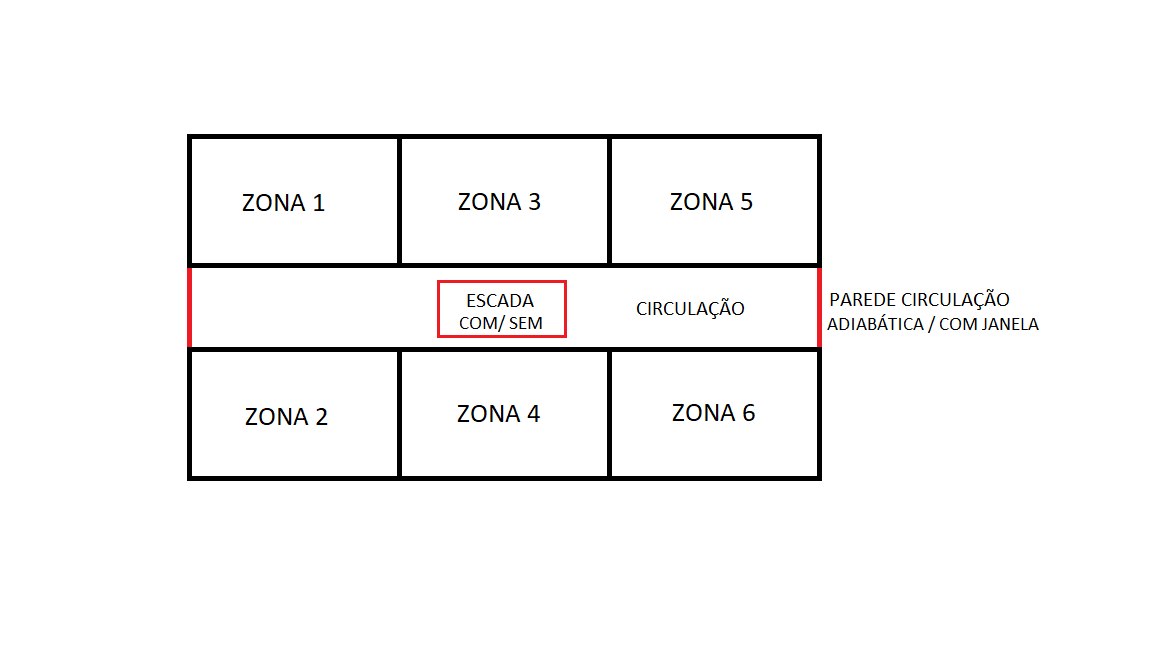
\includegraphics[width=1\linewidth]{img/CROQUI.png}
		\label{fig:croqui}
	\end{figure}
	\begin{flushleft}
		Fonte: o autor.
	\end{flushleft}
	
	Devido a limitações na obtenção dos coeficientes de pressão para as faces externas da edificação, as edificações modeladas terão sempre formato retangular.
	
	A partir dessa tipologia, serão definidas diferentes proporções geométricas, levando-se em consideração a largura, profundidade, altura da edificação e o pé-direito. Também serão parametrizados a altura do pavimento e a orientação da edificação.
	
	As aberturas do modelo também serão variadas. Cada sala terá uma porta. Salas com apenas uma fachada, possuirão uma janela; salas com duas fachadas poderão possuir uma ou duas janelas. As janelas modeladas possuirão diferentes frações de abertura para representar diferentes modelos de janela tipicamente encontrados nas edificações de escritórios. As dimensões das janelas também serão variadas. Além da área da abertura ter influência direta nas trocas de ar das zonas, a altura também pode ter influência devido à força de empuxo causada pelas diferenças de densidade do ar. Devido a isso, a altura da janela também será variada. Para o vidro das janelas, diferentes materiais serão utilizados, variando-se sua transmitância e fator solar.
	
	A variação nas propriedades termofísicas da envoltória representará diferentes materiais construtivos, possibilitando a descrição de uma quantidade significativa do universo de casos aplicáveis às edificações de escritórios consideradas. Serão variadas a transmitância térmica, capacidade térmica e absortância. Os pisos e as lajes entre pavimentos serão considerados como lajes de concreto com piso cerâmico, com as propriedades térmicas apresentadas na Tabela 3.3. As coberturas serão modeladas como laje de cimento e telhado de fibrocimento, separadas por uma câmara de ar. As propriedades térmicas da cobertura também estão apresentadas na Tabela 3.3. Como apenas um pavimento é modelado, pisos e tetos de pavimentos intermediários são considerados adiabáticos.
	
	\section{Ventilação natural}
	
	A ventilação natural será modelada a partir do modelo AirflowNetwork (AFN) do EnergyPlus (DOE, 2018).
	
	O controle das janelas será estabelecido pela diferença de temperatura entre o ar externo e o ar da zona. As trocas de ar nas portas ocorrerão apenas por frestas, por considerar-se que portas de escritórios não ficam abertas normalmente.
	
	Os coeficientes de pressão nos nós externos à edificação serão definidos através da base de dados de Tokyo (TPU, 2018), e para cada janela será utilizado o valor médio dos pontos disponíveis para sua área na fachada, de acordo com a Figura X.
	
	\section{Modelo simplificado}
	
	O objetivo de gerar um modelo de RNA para se obter o EHF faz com que se busque parametrizar ao máximo os modelos desenvolvidos no Energyplus. Essa parametrização pode facilitar o desenvolvimento de amostras para a pesquisa, assim como garantir uma relação mais direta dos parâmetros de entrada com os dados de saída. Portanto, nesta etapa do método busca-se simplificar e parametrizar o modelo de escritório desenvolvido no Energyplus, atentando-se às limitações relacionadas à simplificação do modelo.
	
	Dentre as simplificações consideradas, estão:
	
	\begin{itemize}
		\item cálculo do Cp através do método analítico, em vez dos dados obtido por medições em túnel de vento pela TPU;
		\item representação dos materiais da envoltória através de duas camadas: uma camada representando a capacidade térmica (concreto), e uma camada para regular a transmitância (objeto Material:NoMass);
		\item modelagem da zona que representa um escritório isoladamente, sem modelar as demais zonas térmicas da edificação. Para isso, são definidas as condições de contorno relacionadas às faces da zona correspondentes a paredes adjacentes à edificação;
		\item definição de um coeficiente de infiltração relacionado à infiltração de ar pela porta, e do valor de Cp relacionado à porta, que está voltada para o corredor, e não para o ambiente externo.`
	\end{itemize}
	
	O impacto nos resultados das simulações serão verificados para cada uma das simplificações mencionadas. Desta forma, será definida a forma mais adequada de simplificar o modelo, assim como a margem de erro que espera-se encontrar ao assumir tais simplificações.
	
	\section{Túnel de vento x Método analítico}
	
	Para verificar o quanto os resultados das simulações são influenciados pela fonte utilizada na definição dos valores de Cp, comparou-se os resultados de ACH e EHF em simulações com valores de Cp obtidos pela base da TPU aos resultados obtidos para simulações com valores de Cp obtidos pelo método analítcio de SwamiShandra(?), que é algoritmo padrão do Energyplus.
	
	Equanto valores de Cp através do método analítco podem ser obtidos pra quaisquer razões entre dimensões das fachadas da edificação, os valores da base TPU são fornecido para edificações com geometrias específicas. Ambas as fontes são limitadas a edificações retangulares.
	
	Para o tipo de edificação simulados neste estudo, a TPU disponibiliza valores de Cp para 25 geometrias diferentes, das quais 13 são para edificações altas (highrise), e 12 são para edificações baixas (lowrise). Para cada uma dessas geometrias disponíveis, valores de Cp são disponibilizados para diversos pontos na fachada da edificação, de acordo com a Figura X.
	
	Para verificar as diferenças nos valores de Cp, calculou-se valores de Cp correspondentes a cada geometria disponível pela TPU através do método analítico, e subtraiu-se o valor de Cp calculado para cada fachada pelos valores disponibilizados pela base da TPU para a fachada correspondente (Equação X).
	
	A partir dessas diferenças entre os valores de Cp, escolheu-se a geometria com a maior média de diferença absoluta para se analisar a influência da diferença desses valores nos resultados das simulações no Energyplus.
	
	O modelo base para verificar as diferenças dos resultados utilizando-se valores de Cp com origens diferentes foi o modelo de pavimento com 6 escritórios. Para evitar a influência do solo e da cobertura, considerou-se um pavimento intermediário. A base da TPU permite a obtenção de diferentes coeficientes de pressão para diferentes janelas, como mencionado na seção anterior. No modelo baseado no método analítico, utilizou-se um valor de Cp por fachada, devido à limitação do método. Uma amostra de 1000 casos foi gerada pelo método de amostragem do hipercubo latino. A amostra gerada teve parâmetros variados de acordo com a Tabela \ref{table:cpmethod}.
	
	\begin{table}[h]
		\centering
		\caption{Descrição da tabela.}
		\label{table:cpmethod}
		\begin{tabular}{|c |c |c |c |}
			\hline
			\textbf{Parâmetro} & \textbf{Unidade} & \textbf{Mínimo} & \textbf{Máximo} \\
			\hline
			Área & m$^2$ & 20 & 100 \\
			\hline
			Pé-direito & m & 2,4 & 3,2 \\
			\hline
			Azimute & graus & 0 & 359,9 \\
			\hline 
			Transmitância & W/m$^2$ & 0,5 & 4,4 \\
			\hline 
			PAF & - & 0,1 & 0,6 \\
			\hline 
			Ocupação & pessoa/m$^2$ & 0,05 & 0,50 \\
			\hline 
			Pavimento & - & 1 & 8 \\
			\hline 
		\end{tabular}
		\begin{flushleft}
			Fonte: ASHRAE Standard 55 (2017)
		\end{flushleft}				
	\end{table}
	
	Para cada caso da amostra, foram simulados um modelo com Cp’s baseados no método analítico, e um modelo com Cp’s baseados na base da TPU (túnel de vento).
	
	\section{Representação da envoltória}
	
	Para possibilitar a parametrização contínua e independente das propriedades termofísicas da envoltória, considerou-se a utilização de uma parede com propriedades equivalentes, modelada com uma camada de concreto, para representar a capacidade térmica, e uma camada modelada com o objeto Material:NoMass, para regular a transmitância.
	A validação da modelagem simplificada da parede foi feita para 3 tipos de parede:
	
	\begin{itemize}
		\item parede de concreto;
		\item parede de alvenaria e reboco;
		\item parede de gesso com lã de rocha.
	\end{itemize}`
	
	Como a modelagem da parede de alvenaria possui uma camada de ar no meio da parede, considerou-se a possibilidade de a capacidade térmica a ser considerada na parede de concreto+eps ser melhor representada considerando-se apenas metade da parede.
	
	Para validar essa simplificação, gerou-se uma amostra utilizando HCL, com 100 casos. O modelo preliminar sofreu variação dos seguintes parâmetros: área, razão entre largura e profundidade da zona, pé-direito, azimute, absortância, PAF, taxa de ocupação.
	
	Cada caso da amostra foi simulado com os três tipos de paredes diferentes, e suas paredes equivalentes. No caso da parede de alvenaria, um modelo de parede equivalente foi desenvolvido considerando-se apenas metade da parede de alvenaria.
	
	A partir dos resultados, observou-se a diferença média entre as temperaturas operativas das zonas nos modelos com as paredes referências em relação aos modelos com as respectivas paredes equivalentes. O mesmo foi feito comparando-se o EHF.
	
	\section{Condição de contorno das paredes adjacentes}
	
	Simular apenas uma zona, em vez de um edifício ou de um pavimento com diversas zonas, possibilita a simulação de muitos casos diversos em menos tempo.
	
	Para modelar apenas uma zona, considerou-se as paredes correspondentes a superfícies voltadas para outros escritórios como adiabáticas. A superfície que representa a parede voltada para o corredor foi testada com duas condições de contorno: como adiabática, e como outdoors, sem incidência de vento ou sol.
	
	O modelo de referência é o modelo preliminar. Para cada caso referência, seis modelos de uma zona foram modelados, correspondendo a cada uma das zonas do modelo referência. A modelagem da ventilação natural sofre um impacto significativo quando o escritório é modelado como apenas uma zona. Esse impacto é devido à forma como a rede de fluxo de ar é montada. No caso do modelo referência, a porta é voltada para o corredor, enquanto que no caso de uma única zona, a porta da zona é voltada para a rua. Além disso, não é possível modelar uma porta em uma parede adiabática. Para não deixar a diferença na ventilação natural influenciar as análises comparativas entre os modelos, a ventilação natural não foi modelada para esta etapa. Em vez disso, os modelos foram desenvolvidos com uma taxa de infiltração de ar constante durante a ocupação. O valor escolhido para a taxa de renovação de ar foi igual ao valor médio obtido na etapa da comparação entre os métodos de obtenção dos valores de Cp, que é igual a 30 ach.
	
	Para validar o uso de diferentes condições de contorno, comparou-se os resultados de EHF e temperaturas operativas das zonas únicas com os modelos referência. A condição de contorno com menores diferenças médias absolutas, foi escolhida para gerar o modelo simplificado.
	
	\section{Modelagem da ventilação natural no modelo simplificado}
	
	A modelagem da ventilação natural no modelo simplificado deve ser adaptada para se ter resultados correspondentes ao esperado em relação aos modelos referência.
	
	No AFN do EnergyPlus não é possível modelar aberturas ou infiltração de ar em superfícies adiabáticas. Para contornar esse problema, no caso de se modelar uma parede voltada para o corredor como adiabática, é possível associar a infiltração referente à porta a uma outra superfície da zona que esteja voltada para o ambiente externo. A solução para isso é modelar diretamente os objetos dos nós relacionados às aberturas dos modelos, ou seja, os coeficientes de pressão. Desta forma é possível definir valores de Cp para superfícies (seja janela ou parede) considerando-se qualquer orientação desejada, e não necessariamente a orientação definida para aquela superfície na geometria do modelo.
	
	A modelagem do fluxo de ar pelas portas dos escritórios nos modelos de zona única foi desenvolvida com o objeto AirflowNetwork:MultiZone:Surface:Crack. O motivo para se utilizar este objeto é porque este é um objeto que pode ser associado a qualquer superfície. Portanto, o objeto crack é associado à parede externa oposta à parede voltada para o corredor.
	
	Esta forma de contornar o problema da infiltração na parede adiabática impede que os valores de Cp sejam calculados automaticamente pelo Energyplus, portanto valores de Cp específicos são calculados para cada abertura do modelo. A fórmula utilizada para calcular os valores de Cp é a mesma do algoritmo padrão do Energyplus, porém a orientação da abertura é alterada conforme desejado.
	
	Além da solução descrita para atribuir adequadamente os valores de Cp às aberturas, existe outra limitação: as diferenças de pressão entre as zonas dos escritórios e do corredor variam de acordo com a direção do vento, mas não de forma igual ao que se calcularia considerando-se o Cp da fachada. Dentro da rede de fluxo do AFN, a pressão do corredor depende das trocas de ar entre todas as zonas adjacentes e as trocas de ar pelas janelas do corredor. Em um modelo de zona única isso não poderia ser incluído. Para tentar contornar este problema, buscou-se uma forma de gerar um Cp equivalente para a porta no modelo de uma única zona. Esse cálculo foi feito considerando-se a equação X. A equação proposta leva em conta as resistências de todas as aberturas da edificação de referência, e calcula uma relação entre as pressões do ar externo e do corredor para cada direção de vento. Essas relações entre as pressões são adotadas então como valores de Cp.
	
	Devido a essas considerações, a validação foi conduzida para duas condições: considerando-se o Cp calculado diretamente pelo método analítico, e considerando-se o Cp equivalente, que leva em conta a relação entre as pressões nas zonas para cada direção de vento.
	
	Estas análises foram conduzidas considerando-se diferentes valores de coeficiente de infiltração para o objeto AirflowNetwork:MultiZone:Surface:Crack, para ajustar o valor mais adequado à taxa de infiltração que se obtém no modelo referência.
	
	%Como as taxas de infiltração são influenciadas pela temperatura do ar, as comparações com os modelos referências foram feitas considerando-se diferentes faixas de temperatura.
	
	\section{Análise de sensibilidade}
	
	Com a definição de como serão gerados os modelos simplificados, uma análise de sensibilidade será aplicada. Através da análise de sensibilidade, a influência das diferentes variáveis nos modelos serão avaliadas. Características parametrizáveis nos modelos preliminares que não sejam relevantes nos resultados de temperatura operativa e, consequentemente, fração de horas de desconforto por calor, serão fixadas.
	
	O método de Sobol (1993) será utilizado para a análise de sensibilidade, pois permite a identificação de parâmetros influentes, mesmo para casos onde a relação entre as entradas e saídas dos modelos são não-monotônicas  e apresentam efeitos colineares. A amostragem para essa análise é definida pelo próprio método. A aplicação será feita através da biblioteca SALib (HERMAN; USHER, 2017), escrita na linguagem Python (PYTHON, 2018). A partir de uma amostra com 99.978 casos, obteve-se índices de sensibilidade para análise de 1ª ordem, 2ª ordem, e total.
	
	\section{Desenvolvimento da rede neural artificial}
	
	A base de dados utilizada para o treinamento do metamodelo foi desenvolvida a partir de XXX.XXX resultados de simulações, amostrados pelo método de amostragem de Sobol. A etapa de validação foi executada com outra amostra de XX.XXX casos, amostrados pelo método do HCL. Na amostra da validação, os parâmetros não incluídos como dados de entrada para a RNA tiveram os valores fixados iguais aos da amostra utilizada para o treinamento. O motivo para se utilizar diferentes métodos de amostragem é para evitar qualquer enviesamento possivelmente relacionado ao método de amostragem.
	
	Após a etapa de validação, a amostra gerada para a AS foi utilizada para verificar o desempenho da RNA quando os valores dos parâmetros não considerados como dados de entrada da RNA variam. A escolha desta 
	
	Após definir quais variáveis do modelo preliminar exigem parametrização, e quais podem ser fixadas, a configuração do modelo base final será definida.
	
	A partir do modelo base final, será desenvolvida uma base de dados através do método de amostragem do Hipercubo Latino.
	
	É importante ressaltar que cada modelo simulado pelo EnergyPlus possuirá diversas zonas térmicas, e que cada zona será considerada como um caso específico para a base de dados utilizada no treinamento da rede neural artificial (RNA). Portanto, cada caso do banco de dados gerado para o treinamento da RNA será um vetor, contendo diversas informações sobre as características da sala, e dos resultados obtidos de fração de horas de calor para esta sala.
	
	O desenvolvimento do metamodelo será por meio do sistema computacional de redes neurais artificiais. Esse processo será executado através da linguagem de programação Python. A RNA será treinada com 80\% da base de dados gerada. A parte restante será utilizada para validação do metamodelo.
	
	A forma como as variáveis descritas nos modelos simulados serão introduzidas no metamodelo a ser desenvolvido podem influenciar a precisão e a representação adequada dos fenômenos termofísicos. No processo de definição das variáveis de entrada do metamodelo, busca-se a melhor forma de descrever as diversas características das salas e do clima. Esse é um processo iterativo, no qual varia-se diferentes variáveis de entrada, utilizando-se às vezes transformações, normalizações e funções destas. É importante também observar os hiper-parâmetros (parâmetros relacionados ao processo de aprendizagem automática) escolhidos na criação da RNA. A precisão da rede pode depender do número de nós, número de camadas, assim como outros parâmetros definidos durante o processo de treinamento.
	
	Para validar a RNA, serão comparados os resultados obtidos através do metamodelo com os casos não vistos da base de dados de simulações do EnergyPlus. Como indicadores de precisão, serão utilizados a raiz quadrada da média dos erros ao quadrado (RMSE) e o coeficiente de determinação (R$^2$).

\chapter{Resultados e Discussões}
\label{chapter:resultados}

Lorem ipsum dolor sit amet, consectetur adipiscing elit. Nulla commodo, augue non consectetur vehicula, felis velit commodo eros, nec bibendum augue purus quis mi. Donec dapibus id magna eget euismod. In lacinia porttitor velit, in lacinia erat commodo et. Nulla feugiat posuere ipsum, eu euismod lorem efficitur ut. Sed dapibus lobortis ex, eu vehicula sem dignissim nec. Phasellus pellentesque tellus vitae tortor consectetur volutpat. Proin pulvinar lectus id tellus congue maximus.

Sed semper arcu at posuere scelerisque. Pellentesque a lorem eu lorem lobortis cursus aliquam ut diam. Ut tristique, lacus eget gravida euismod, ante nisl elementum elit, a efficitur neque est eu tellus. Phasellus in convallis tortor. Nullam auctor auctor tempus. Pellentesque placerat, est at convallis congue, velit sapien tempor orci, eu eleifend nisi purus sed odio. Duis nec rhoncus enim. Nunc vitae consectetur sapien. Nullam in enim iaculis, laoreet ex in, aliquet massa. Nulla facilisi. Sed vulputate eros et mi imperdiet, nec commodo libero tristique. Mauris vel pretium felis. Suspendisse feugiat tortor vitae dapibus semper. Fusce dignissim est eget mattis auctor.

Aenean ultrices feugiat faucibus. Sed ut vehicula ligula, vitae pulvinar enim. Ut vel consectetur dolor, a eleifend mauris. Pellentesque tristique justo id felis consectetur pulvinar. Phasellus diam felis.

\chapter{Conclusões}
\label{chapter:conclusoes}
	
Lorem ipsum dolor sit amet, consectetur adipiscing elit. Nulla commodo, augue non consectetur vehicula, felis velit commodo eros, nec bibendum augue purus quis mi. Donec dapibus id magna eget euismod. In lacinia porttitor velit, in lacinia erat commodo et. Nulla feugiat posuere ipsum, eu euismod lorem efficitur ut. Sed dapibus lobortis ex, eu vehicula sem dignissim nec. Phasellus pellentesque tellus vitae tortor consectetur volutpat. Proin pulvinar lectus id tellus congue maximus.

Sed semper arcu at posuere scelerisque. Pellentesque a lorem eu lorem lobortis cursus aliquam ut diam. Ut tristique, lacus eget gravida euismod, ante nisl elementum elit, a efficitur neque est eu tellus. Phasellus in convallis tortor. Nullam auctor auctor tempus. Pellentesque placerat, est at convallis congue, velit sapien tempor orci, eu eleifend nisi purus sed odio. Duis nec rhoncus enim. Nunc vitae consectetur sapien. Nullam in enim iaculis, laoreet ex in, aliquet massa. Nulla facilisi. Sed vulputate eros et mi imperdiet, nec commodo libero tristique. Mauris vel pretium felis. Suspendisse feugiat tortor vitae dapibus semper. Fusce dignissim est eget mattis auctor.

Aenean ultrices feugiat faucibus. Sed ut vehicula ligula, vitae pulvinar enim. Ut vel consectetur dolor, a eleifend mauris. Pellentesque tristique justo id felis consectetur pulvinar. Phasellus diam felis.


\section{Limitações e justificativas}

As limitações desse estudo são indicadas em conformidade com a ordem de execução das etapas de desenvolvimento:

\begin{itemize}
	\item Lorem ipsum dolor sit amet, consectetur adipiscing elit. Nulla commodo, augue non consectetur vehicula, felis velit commodo eros, nec bibendum augue purus quis mi. Donec dapibus id magna eget euismod;
	
	\item Lorem ipsum dolor sit amet, consectetur adipiscing elit. Nulla commodo, augue non consectetur vehicula, felis velit commodo eros, nec bibendum augue purus quis mi. Donec dapibus id magna eget euismod;
	
	\item Lorem ipsum dolor sit amet, consectetur adipiscing elit. Nulla commodo, augue non consectetur vehicula, felis velit commodo eros, nec bibendum augue purus quis mi. Donec dapibus id magna eget euismod.
	
\end{itemize}

\section{Sugestões para trabalhos futuros}

As sugestões para trabalhos futuros são indicadas em conformidade com as potencialidades expressas nesse estudo, sendo:

\begin{itemize}
	\item Lorem ipsum dolor sit amet, consectetur adipiscing elit. Nulla commodo, augue non consectetur vehicula, felis velit commodo eros, nec bibendum augue purus quis mi. Donec dapibus id magna eget euismod;

	\item Lorem ipsum dolor sit amet, consectetur adipiscing elit. Nulla commodo, augue non consectetur vehicula, felis velit commodo eros, nec bibendum augue purus quis mi. Donec dapibus id magna eget euismod;

	\item Lorem ipsum dolor sit amet, consectetur adipiscing elit. Nulla commodo, augue non consectetur vehicula, felis velit commodo eros, nec bibendum augue purus quis mi. Donec dapibus id magna eget euismod.
	
\end{itemize}

\begin{appendices}
	\chapter{Classificação climática de Köppen-Geiger}
	\begin{figure}[!h]
		\centering
		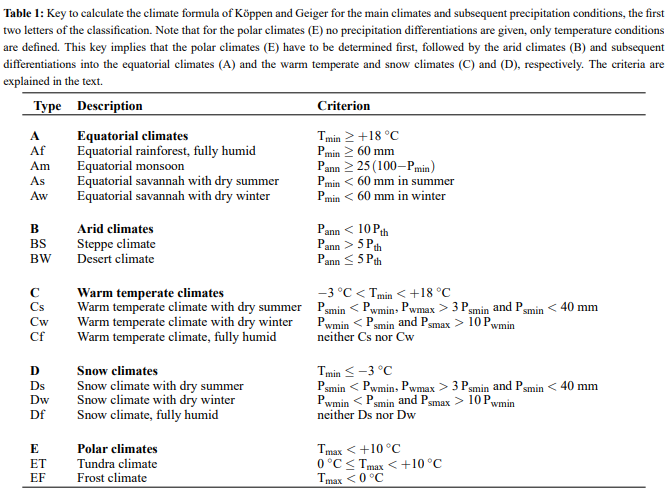
\includegraphics[width=1\linewidth]{img/tablekoppengeiger1.png}
		\label{fig:tablekoppengeiger1}
	\end{figure}
\end{appendices}

\begin{appendices}
	\chapter{Código...}
	\lstset{language=c++}
	\lstset{label={lst:code_direct}}
	\lstset{basicstyle=\tiny}	
	\lstinputlisting{code/code.cc}
\end{appendices}

%\bibliographystyle{lib/abntex2-num}
%\bibliographystyle{lib/abntex2-alf}
\bibliography{citacoes}
	
\end{document}